\chapter[Personalized Schedules for Burdensome Surveillance Tests][Personalized Schedules for Burdensome Surveillance Tests]{Personalized Schedules for Burdensome Surveillance Tests}
\label{c4}

\vspace*{\fill}
\textbf{This chapter is based on the paper}\\
\underline{Tomer, A.}, Nieboer, D., Roobol, M.J., Steyerberg, E.W., and Rizopoulos, D. (2020), Personalized schedules for burdensome surveillance tests. Submitted to \emph{Journal of the American Statistical Association}

\clearpage
\begin{abstract}
Benchmark surveillance \textit{tests} for diagnosing disease \textit{progression} (e.g., biopsies, endoscopies) in early-stage chronic non-communicable diseases (e.g.,~cancer, lung diseases) are usually invasive. For detecting progression timely, patients undergo invasive tests planned in a fixed one-size-fits-all manner (e.g.,~annually). We present personalized test schedules based on progression-risk, that aim to optimize the number of tests (burden) and time delay in detecting progression (shorter is beneficial) better than fixed schedules. Our motivation comes from the problem of scheduling biopsies in prostate cancer surveillance.

Using joint models for time-to-event and longitudinal data, we consolidate patients' longitudinal data (e.g.,~biomarkers) and results of previous tests, into individualized future cumulative-risk of progression. We then create personalized schedules by planning tests on future visits where the predicted cumulative-risk is above a \textit{threshold} (e.g.,~5\% risk). We update personalized schedules with data gathered over follow-up. To find the optimal risk threshold, we minimize a utility function of the expected number of tests (burden) and expected time delay in detecting progression (shorter is beneficial) for different thresholds. We estimate these two in a patient-specific manner for following any schedule, by utilizing a patient's predicted risk profile. Patients/doctors can employ these quantities to compare personalized and fixed schedules objectively.
\end{abstract}
\clearpage
% !TEX root =  ../main_manuscript.tex 
\section{Introduction}
\label{c4:sec:introduction}
Chronic non-communicable diseases (e.g., cancer, lung, cardiovascular diseases) cause 60--70\% of human deaths worldwide~\citep{world2014global}. Often patients diagnosed with an early-stage disease undergo surveillance \emph{tests} to detect disease \emph{progression} timely. A progression is a non-terminal event, and usually a trigger for treatment and/or removal from surveillance. Benchmark tests used for confirming progression are usually \emph{invasive}, e.g., biopsies in prostate cancer surveillance~\citep{bokhorst2015compliance}, endoscopies in Barrett's esophagus~\citep{weusten2017endoscopic}, colonoscopies in colorectal cancer~\citep{krist2007timing}, and bronchoscopies in post lung transplant~\citep{mcwilliams2008surveillance} surveillance.

Invasive tests are repeated until progression is observed, typically as per a one-size-fits-all \emph{fixed schedule}, e.g., biannually,~\citep{krist2007timing,mcwilliams2008surveillance,bokhorst2015compliance}. A time gap between tests causes a time delay in detecting progression (Figure~\ref{c4:fig:1}). A shorter delay in detecting progression (\emph{benefit}) can provide a larger window of opportunity for curative treatment. However, with fixed schedules, this means conducting tests frequently. Frequent tests are \textit{burdensome} as they may cause pain and/or severe medical complications~\citep{krist2007timing,loeb2013systematic}. Consequently, patients may not always comply with frequent tests~\citep{bokhorst2015compliance, LeClercq2015325}. In general, because fixed schedules do not differentiate between fast and slow/non-progressing patients, they impose disproportionate burden/benefits across the patient population.

\begin{figure}
\centerline{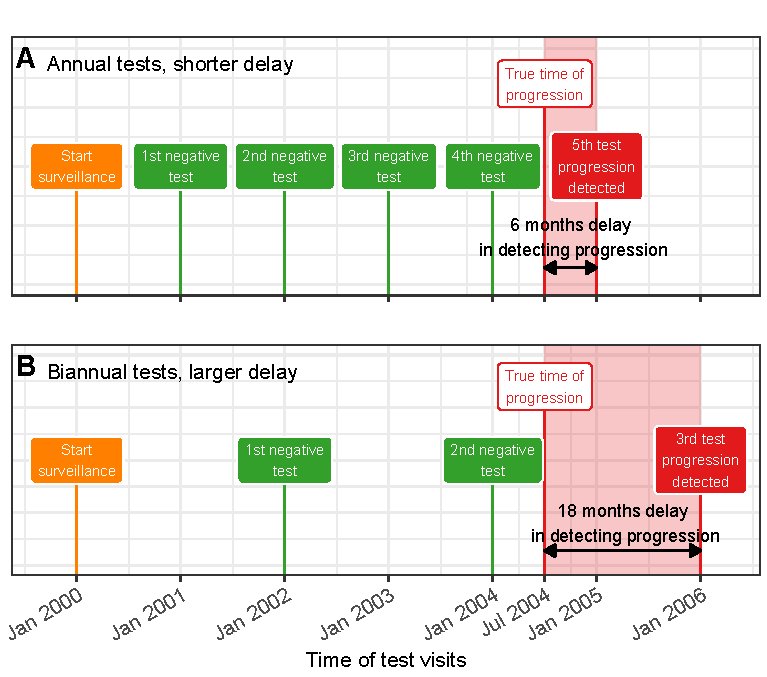
\includegraphics{contents/c4/images/c4_fig1.pdf}}
\caption{\textbf{Goal: Finding the optimal tradeoff between the number of invasive tests (burden) and time delay in detecting progression (shorter is beneficial)}. A progression is a non-terminal event in the surveillance of early-stage chronic non-communicable diseases. The true time of progression for the patient illustrated in this figure is July 2004. Since invasive tests are conducted repeatedly, progression is interval-censored and always observed with a delay. Frequent periodical invasive tests in \textbf{Panel~A} lead to a shorter time delay in detecting progression than infrequent periodical invasive tests in \textbf{Panel~B}. The interval-censored time of progression is Jan~2004--Jan~2005 in \textbf{Panel~A} and between Jan~2004--Jan~2006 in \textbf{Panel~B}.}
\label{c4:fig:1}
\end{figure}

The goal of this work (Figure~\ref{c4:fig:1}) is to optimize the number of invasive tests (burden) and the time delay in detecting progression (shorter is beneficial) better than fixed schedules. Specifically, we intend to \emph{personalize} test schedules using patients' clinical data accumulated over surveillance follow-up. This data includes baseline characteristics, previous test results, and longitudinal outcomes (e.g., biomarkers, medical imaging, physical examination). Many surveillance protocols currently personalize test schedules using heuristic methods such as decision flowcharts~\citep{bokhorst2015compliance,weusten2017endoscopic}. However, flowcharts discretize continuous outcomes, often exploit only the last measurement, ignore the measurement error in observed data, and plan only one test at a time. Alternatively, a complete personalized schedule of tests can be obtained using partially observable Markov decision processes or POMDPs~\citep{alagoz2010operations,steimle2017markov}. Although POMDPs typically discretize continuous longitudinal outcomes to avoid the curse of dimensionality. In scenarios such as ours, where decisions (test/no test) and disease state (low-grade disease/progressed) are both binary, POMDPs may not be necessary either. The reason is that such POMDPs give the same optimal schedule, which can be alternatively obtained by just planning a test when the probability of transition from non-progressed to progressed state is more than a certain threshold~\cite[see][Equation~1]{vickers2006decision}. 

Personalized schedules can also be obtained by optimizing an explicit utility function of the burden and/or benefit of a schedule. A challenge in this approach is quantifying burden and benefit. For a single test decision, \citet{tomer2019personalizedbiometrics} quantify the burden and benefit as the time difference by which the test undershoots (unnecessary test) or overshoots (delayed detection) the true progression time of a patient, respectively. Whereas, for a complete test schedule, \citet{bebu2017optimal} quantify burden as the number of tests planned (or their cost), and benefit as short time delay in detecting progression. Although, unlike the number of tests, the costs of time delay in detecting progression are not always quantifiable. For this issue, \citet{bebu2017optimal}, and \citet{vickers2006decision} have proposed scheduling tests when the risk of progression is above a threshold. Risk-based methodologies has also been explored by \citet{rizopoulos2015personalized}, and to evaluate the choice of risk thresholds \citet{wang2019learning} and \citet{tomer2019personalized} use measures of diagnostic accuracy (e.g., false-positive rate, true positive rate). However, a limitation of risk-based test decisions is that a single decision does not inform patients about the clinical consequences of continuing on surveillance. Also, measures of diagnostic accuracy are not personalized criteria for choosing risk thresholds.

We improve upon the works referenced above in many ways. Instead of a single risk-based test decision, we derive full risk-based test schedules that dynamically update with new clinical data over follow-up. Along with each schedule, we provide patients the clinical consequences of following it. Namely, the expected number of tests that will be required out of all planned tests to detect progression and the expected time delay in detecting progression. Unlike measures of diagnostic accuracy, we calculate these in a personalized manner. Also, these two are easily-quantifiable surrogates for important clinical aspects such as the window of opportunity for curative treatment, risk of adverse outcomes due to delayed detection of progression, financial costs of tests, risk of side-effects, and reduction in quality of life, etc. Our methodology is as follows. We first develop a full specification of the joint distribution of the patient-specific longitudinal outcomes and the time of progression. To this end, we utilize joint models for time-to-event and longitudinal data~\citep{tsiatis2004joint,rizopoulos2012joint} because they are inherently personalized. Specifically, joint models utilize patient-specific random effects~\citep{mcculloch2005generalized} to model longitudinal outcomes without discretizing them. Subsequently, we input clinical data of a new patient into the fitted model to obtain their predicted patient-specific cumulative-risk of progression at future visits. We then create personalized schedules by planning tests on future visits where this predicted cumulative-risk is above a particular \emph{threshold} (e.g., 5\% risk). We automate the choice of this threshold and the resulting schedule. In particular, we optimize a utility function of the expected number of tests (burden) and time delay in detecting progression (shorter is beneficial) for personalized schedules. We estimate these two quantities for any given schedule in a patient-specific manner using the patient's predicted risk profile. Hence, patients/doctors can compare the consequences of opting for personalized versus fixed schedules objectively.

Our motivation comes from the problem of scheduling biopsies in the world's largest prostate cancer surveillance study, called Prostate Cancer Research International Active Surveillance~\citep{bokhorst2015compliance}, or PRIAS. It has 7813 low/very-low grade cancer patients (1134 progressions, 104904 longitudinal measurements), many of whom are potentially over-diagnosed due to prostate-specific antigen (PSA) based screening~\citep{loeb2014overdiagnosis}. To reduce subsequent over-treatment, in surveillance, serious treatments (e.g., surgery, radiotherapy) are delayed until progression is observed. Surveillance involves regular monitoring of a patient's PSA (ng/mL), digital rectal examination or DRE (tumor shape/size), and biopsy Gleason grade group~\citep{epsteinGG2014}. Among these, a biopsy Gleason grade group~$\geq$ 2 is the reference test for confirming progression. Most often, biopsies are scheduled annually~\citep{loeb2014heterogeneity}. However, such a frequent schedule can put an unnecessary burden on patients with slow/non-progressing cancers and cause non-compliance~\citep{bokhorst2015compliance}. Since prostate cancer has the second-highest incidence among all cancers in males~\citep{GlobalCancerStats2012}, individualized biopsy schedules can reduce the burden of biopsies in numerous patients worldwide.

The remaining paper is as follows. Section~\ref{c4:sec:jointmodel} introduces the joint modeling framework. We describe the personalized scheduling methodology in Section~\ref{c4:sec:schedule}, and demonstrate them for prostate cancer surveillance patients in Section~\ref{c4:sec:results}. In Section~\ref{c4:sec:sim_study}, we compare personalized and fixed schedules via a simulation study based on a joint model fitted to the PRIAS dataset.
\section{Joint Model for Time-to-Progression and Longitudinal Outcomes}
\label{c4:sec:jointmodel}
Text currently under embargo.
% !TEX root =  ../main_manuscript.tex 
\section{Personalized Schedule of Invasive Tests for Detecting Progression} 
\label{c4:sec:schedule}

\subsection{Cumulative-risk of progression} 
\label{c4:subsec:cum_risk}
Text currently under embargo.

\subsection{Personalized Test Decision Rule} 
\label{c4:subsec:pers_schedule}
Text currently under embargo.

\subsection{Expected Number of Tests and Expected Time Delay in Detecting Progression}
\label{c4:subsec:exp_delay_estimation}
Text currently under embargo.

\subsection{How to Select the Risk Threshold~$\kappa$}
\label{c4:subsec:kappa_selection}
Text currently under embargo.
\section{Application of Personalized Schedules in Prostate Cancer Surveillance}
\label{c4:sec:results}
We next demonstrate personalized schedules for scheduling biopsies in prostate cancer active surveillance. To this end, we use results from a joint model fitted to the PRIAS dataset introduced in Section~\ref{c4:sec:introduction}. The model definition (Appendix~\ref{c4:appendix:prias_model}) utilized a linear mixed sub-model for biannually measured PSA (continuous: log-transformed from ng/mL), and a logistic mixed sub-model for biannually measured DRE (binary: tumor palpable or not). In the survival sub-model, fitted PSA value, fitted instantaneous PSA velocity (defined in Section~\ref{c4:subsec:surival_sub_model}), and log-odds of having a DRE indicating a palpable tumor, were included as time-dependent predictors. The model parameters were estimated under the Bayesian framework using the R package \textbf{JMbayes}~\citep{rizopoulosJMbayes}, and are presented in Appendix~\ref{c4:appendix:prias_model}. We next briefly present the key results relevant for personalized scheduling.

First, the cause-specific cumulative-risk of cancer progression at the maximum study period of ten years was 50\% (Figure~\ref{c4:fig:app1}). This indicates that many patients may not require all of the yearly biopsies they are usually prescribed. Since personalized schedules are risk-based, their overall performance is dependent on the predictive accuracy and discrimination capacity of the fitted model. In this regard, the model had a moderate time-dependent area under the receiver operating characteristic curve or AUC~\citep{landmarking2017} over the follow-up period (between 0.61 and 0.68). The time-dependent mean absolute prediction error or MAPE~\citep{landmarking2017} was moderate to large (between 0.08 and 0.24) and decreased rapidly after year one of the follow-up. Thus, personalized schedules based on this model may work better after year one with more follow-up data. Details on AUC and MAPE are provided in Appendix~\ref{c5:appendix:validation}.

\subsection{Personalized Biopsy Schedules for a Demonstration Prostate Cancer Patient}
\label{c4:subsec:demo_patient}
We utilized the joint model fitted to the PRIAS dataset to schedule biopsies in a demonstration prostate cancer patient shown in Figure~\ref{c4:fig:5}. The time of his last negative biopsy was $t=3.5$ years, and the time of the current visit was $v=5$ years. We made biopsy decisions over his future visits for PSA measurement $U=\{u_1=5, u_2=5.5,\ldots,u_L=10\}$ years using four different schedules. Two of the fixed schedules are annual biopsy schedule and the PRIAS schedule. The PRIAS schedule has compulsory biopsies at year one, four, seven, and ten of follow-up, and additional annual biopsies if PSA doubling-time~\citep{bokhorst2015compliance} is high. Remaining two schedules are personalized, namely, with a fixed threshold $\kappa=10\%$ risk, and an automatically chosen current visit time $v$ specific risk $\kappa^*(v)$ (Section~\ref{c4:subsec:kappa_selection}). Since the demonstration patient's time of last negative biopsy $t=3.5$ is after year one of follow-up, a time delay in detecting progression
up to three years may not lead to adverse downstream outcomes~\citep{carvalho}.

\begin{figure}
\centerline{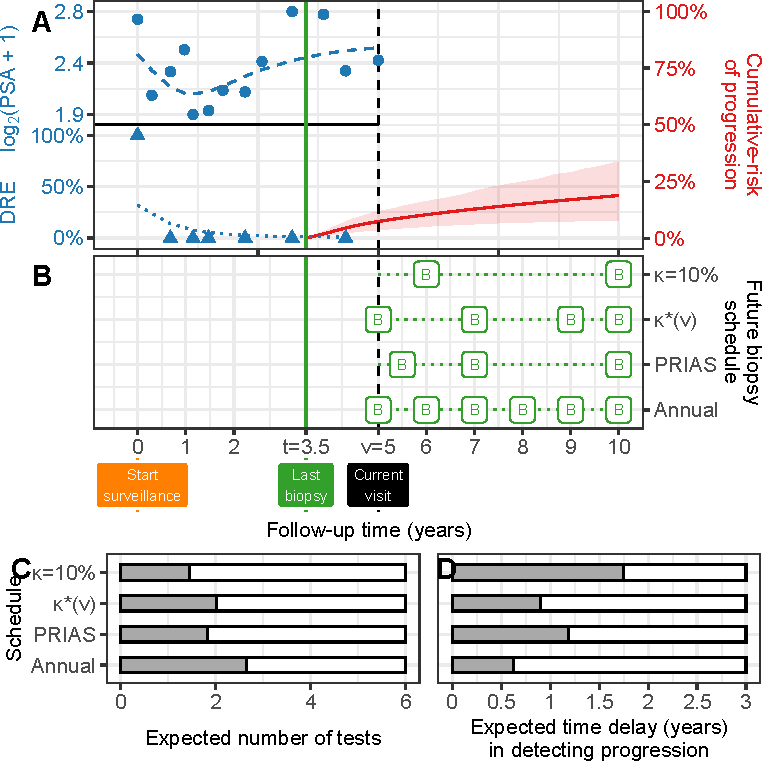
\includegraphics{contents/c4/images/c4_fig5.pdf}}
\caption{\textbf{Personalized schedules for a demonstration prostate cancer patient}. \textbf{Panel~A}: Current visit:~$v=5$ years. Last negative biopsy:~$t=3.5$ years. Longitudinal data:~$\log_2(\mbox{PSA} + 1)$ transformed~\citep{tomer2019personalized} PSA (observed: blue dots, fitted: dashed blue line), binary DRE (observed: blue triangles, fitted probability: dotted blue line). Cumulative-risk profile: solid red line (95\% credible interval shaded). \textbf{Panel~B}: `B' indicates a planned biopsy. \textbf{$\kappa=10\%$} and \textbf{$\kappa^*(v)$} are personalized biopsy schedules using a risk threshold of 10\%, and a visit time~$v$ specific automatic threshold~(\ref{c4:eq:kappa_choice}), respectively. PRIAS biopsy schedule is defined in Section~\ref{c4:subsec:demo_patient}. \textbf{Panel~C,D}: For all schedules we calculate the expected number of tests and expected time delay in detecting progression if the patient progresses before year ten. With a recommended minimum gap of one year between biopsies, maximum possible number of tests are six.}
\label{c4:fig:5}
\end{figure}

The cumulative-risk of progression of the demonstration patient increases 3\% yearly on average, up to 19\% at the maximum study period of ten years. Hence, the patient may progress slowly. Consequently, risk-based personalized approaches plan fewer biopsies than the annual schedule (Panel~B, Figure~\ref{c4:fig:5}). Also, the time delay in detecting progression for personalized schedules (Panel~D, Figure~\ref{c4:fig:5}) is below the safe limit of three years mentioned earlier. Thus, personalized schedules can be a suitable alternative to the annual schedule.
\section{Simulation Study}
\label{c4:sec:sim_study}
Although we evaluated personalized schedules for a demonstration patient, we also intend to analyze and compare personalized and fixed schedules in a full cohort. Our criteria for comparison of schedules are the total number of invasive tests planned (burden), and the actual time delay in detecting progression (shorter is beneficial) for each schedule. Due to the periodical nature of schedules, the actual time delay in detecting progression cannot be observed in real-world surveillance. Hence, instead, we compare personalized versus fixed schedules via an extensive simulated randomized clinical trial in which each hypothetical patient undergoes each schedule. To keep our simulation study realistic, we employ the prostate cancer active surveillance scenario. Specifically, our simulated population is generated using the joint model fitted to the PRIAS cohort (Appendix~\ref{c4:appendix:param_estimates}).

\subsection{Simulation Setup}
From the simulation population, we first sample 500 datasets, each representing a hypothetical prostate cancer surveillance program with 1000 patients in it. We generate a true cancer progression time for each of the ${\mbox{500} \times \mbox{1000}}$ patients, and then sample longitudinal DRE and PSA measurements biannually (PRIAS protocol) for them. We split each dataset into training (750 patients) and test (250 patients) parts, and generate a random and non-informative censoring time for the training patients. All training and test patients also observe Type-I censoring at year ten of follow-up (current study period of PRIAS). We next fit a joint model of the same specification as the model fitted to PRIAS (Appendix~\ref{c4:appendix:param_estimates}), to each of the 500 training datasets and retrieve MCMC samples from the 500 sets of the posterior distribution of the parameters. In each of the 500 hypothetical surveillance programs, we utilize the corresponding fitted joint models to obtain the cumulative-risk of progression in each of the ${\mbox{500} \times \mbox{250}}$ test patients. These cumulative-risk profiles are further used to create personalized biopsy schedules for the test patients. 

For each test patient, we conduct hypothetical biopsies using two fixed (PRIAS and annual schedule) and three personalized biopsy schedules. Personalized schedules are based on, a fixed risk threshold $\kappa=10\%$, an optimal current visit time $v$ specific threshold $\kappa^*(v)$ chosen via~(\ref{c4:eq:kappa_choice}), and an optimal threshold obtained under the constraint that expected time delay in detecting progression is less than 0.75 years (9 months), denoted $\kappa^*\{v \mid E(\mathcal{D})\leq 0.75\}$. The choice of 0.75 years delay constraint is arbitrary and is only used to illustrate that applying the constraint limits the average delay at 0.75 years. Successive personalized biopsy decisions are made only on the standard PSA follow-up visits, utilizing clinical data accumulated only until the corresponding current visit time~(\ref{c4:eq:personalized_decision_grid}). We maintain a minimum recommended gap of one year between consecutive prostate biopsies~\citep{bokhorst2015compliance} as well. Biopsies are conducted until progression is detected, or the maximum follow-up period at year ten (horizon) is reached. The actual time delay in detecting progression is equal to the difference in time at which progression is detected and the actual (simulated) time of progression of a patient.

\subsection{Simulation Results}
In the simulation study, nearly 50\% of the patients observed progression during the ten year study period (\emph{progressing}) and 50\% did not (\emph{non-progressing}). While we can calculate the total number of biopsies scheduled in all $500 \times 250$ test patients, the actual time delay in detecting progression is available only for progressing patients. Hence, we show the simulation results separately for progressing and non-progressing patients (Figure~\ref{c4:fig:6}).

Before discussing delay in detecting progression (Panel~A, Figure~\ref{c4:fig:6}), we note that mean delay up to 1.7 years in all patients~\citep{inoue2018comparative}, and up to three years in patients who progress after year one of follow-up~\citep{carvalho}, may not increase risks of adverse outcomes later. In this regard, the annual biopsies guarantee a maximum delay of one year in all patients. However, they also schedule the highest number of biopsies (Median~3, Inter-quartile range or IQR:~1--6). Much fewer biopsies are planned by the PRIAS schedule (Median~2, IQR:~1--4), but it also has a higher time delay (Median~0.74, IQR: 0.38--1.00 years). The personalized schedule based on optimal risk threshold $\kappa^*(v)$ schedules fewer biopsies than PRIAS and has a delay~(Median~0.86, IQR:~0.46--1.26 years) slightly higher than PRIAS. The expected delay for risk threshold optimized with a constraint on expected delay $\kappa^*\{v \mid E(D)\leq 0.75\}$ is equal to 0.61 years, i.e., the constraint works as expected.

The simulated non-progressing patients (Panel~B,~Figure~\ref{c4:fig:6}) gained the most with personalized schedules. The annual schedule plans 10 (unnecessary) biopsies for each such patient, and the PRIAS schedule plans a median of 6~(IQR:~4--8) biopsies. In contrast, the personalized schedule based on optimized risk threshold $\kappa^*(v)$ plans fewer biopsies consistently (Median~6, IQR:~6--7). The 10\% threshold based schedule plans even fewer biopsies (Median~5, IQR:~4--6).

\begin{figure}
\centerline{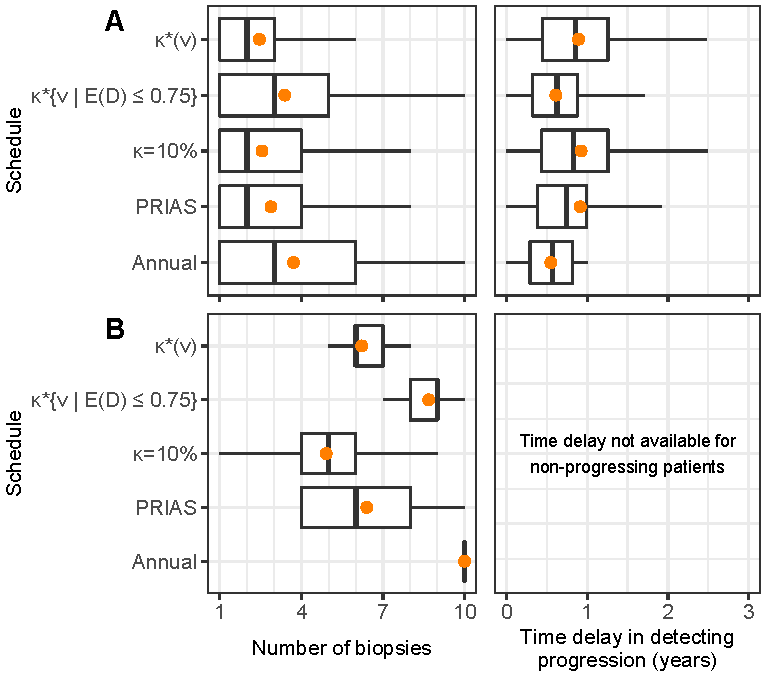
\includegraphics{contents/c4/images/c4_fig6.pdf}}
\caption{\textbf{Number of biopsies and the time delay in detecting cancer progression for various biopsy schedules} obtained via a simulation study. \textbf{Mean} is indicated by the orange circle. Time delay (years) is calculated as (time of positive biopsy - the actual simulated time of cancer progression). Biopsies are conducted until cancer progression is detected. \textbf{Panel~A:} simulated patients who obtained cancer progression in the ten year study period (progressing). \textbf{Panel~B:} simulated patients who did not obtain cancer progression in the ten year study period (non-progressing). Types of schedules: ${\kappa=10\%}$ and $\kappa^*(v)$ schedule a biopsy if the cumulative-risk of cancer progression at the current visit time $v$ is more than 10\%, and an automatically chosen threshold~(\ref{c4:eq:kappa_choice}), respectively. Schedule ${\kappa^*\{v \mid E(\mathcal{D})\leq 0.75\}}$ is similar to $\kappa^*(v)$ except that the euclidean distance in~(\ref{c4:eq:kappa_choice}) is minimized under the constraint that expected delay in detecting progression is at most 9 months (0.75 years). Annual corresponds to a schedule of yearly biopsies, and PRIAS corresponds to biopsies as per PRIAS protocol (Section~\ref{c4:sec:results}).}
\label{c4:fig:6}
\end{figure}
\section{Discussion}
\label{c4:sec:discussion}
Text currently under embargo.

\paragraph{Acknowledgements}
The first and last authors would like to acknowledge support by Nederlandse Organisatie voor Wetenschappelijk Onderzoek (the national research council of the Netherlands) VIDI grant nr. 016.146.301, and Erasmus University Medical Center funding. Part of this work was carried out on the Dutch national e-infrastructure with the support of SURF Cooperative. The authors also thank the Erasmus University Medical Center's Cancer Computational Biology Center for giving access to their IT-infrastructure and software that was used for the computations and data analysis in this study. Last, we would like to thank the PRIAS consortium for enabling this research project.

\section*{Appendix}

\begin{subappendices}
\section{Parameter Estimation}
\label{c4:appendix:param_estimation}
Text currently under embargo.

\section{Joint Model for the PRIAS Dataset Used in Simulation Study}
Text currently under embargo.

\subsection{Model Specification}
Text currently under embargo.

\subsection{Parameter Estimates}
\label{c4:appendix:param_estimates}
Text currently under embargo.

\section{Risk Based Schedules Versus All Possible Schedules}
\label{c4:appendix:all_possible}
Text currently under embargo.

\section{Simulation Study Extended Results}
Text currently under embargo.

\section{Partially Observable Markov Decision Processes}
\label{c4:appendix:pomdp}
Text currently under embargo.

\subsection{Choice of Reward Function for POMDPs}
Text currently under embargo.

\section{Source Code}
\label{c4:appendix:source_code}
Text currently under embargo.

\end{subappendices}

\clearpage
\bibliographystyle{apalike}
\bibliography{c4_bib}